\documentclass[11pt,a4paper]{article}
\usepackage[margin=24mm]{geometry}
\usepackage[T1]{fontenc}
\usepackage{lmodern,amsmath,amssymb,amsthm,mathtools,booktabs,array,graphicx,microtype,enumitem,fancyhdr}
\usepackage[dvipsnames]{xcolor}
\usepackage[colorlinks=true,linkcolor=MidnightBlue,urlcolor=MidnightBlue,citecolor=MidnightBlue]{hyperref}
\usepackage{bookmark}
\setlength{\parindent}{0pt}\setlength{\parskip}{5pt}
\setlist{itemsep=3pt,topsep=4pt}
\pagestyle{fancy}\fancyhf{}
\fancyhead[L]{\small Astra research return | Control speed and quantum access}
\fancyhead[R]{\small 5 November 2026}
\fancyfoot[C]{\thepage}\setlength{\headheight}{14pt}
\newtheorem{theorem}{Theorem}
\newtheorem{lemma}[theorem]{Lemma}
\newcommand{\id}{\operatorname{id}}
\newcommand{\Tr}{\operatorname{Tr}}
\newcommand{\Ad}{\operatorname{Ad}}
\newcommand{\norm}[1]{\left\lVert #1\right\rVert}
\newcommand{\ket}[1]{\lvert #1\rangle}
\newcommand{\bra}[1]{\langle #1\rvert}
\newcommand{\Pcal}{\mathcal P}
\newcommand{\Ncal}{\mathcal N}
\newcommand{\Kcal}{\mathcal K}
\newcommand{\Zcal}{\mathcal Z}
\newcommand{\Gcal}{\mathcal G}
\newcommand{\Lcal}{\mathcal L}
\begin{document}
\hypersetup{pageanchor=false}
\begin{titlepage}
\vspace*{12mm}
{\Large\color{MidnightBlue} ASTRA SCIENTIFIC RETURN\par}
\vspace{10mm}
{\huge\bfseries A control-speed law for reading\newline unencoded quantum systems\par}
\vspace{6mm}
{\Large All finite control strengths, hidden dephasing,\newline and matching local measurement costs\par}
\vspace{9mm}
{\large 5 November 2026, Australia/Brisbane\par}
\vspace{10mm}
\textbf{Question resolved.} Can a protected quantum computer acquire selected global information from an initially unencoded experiment with polynomially many specimens when source interactions act on a fixed number of sites and their speed is only a fixed multiple of the hidden dephasing rate?

\textbf{Completed result.} Under the explicit access contract in this report, the answer is no at every fixed finite control-to-noise ratio, including strong control. A finite-window proof gives an exponential copy lower bound. An explicit local reader matches its scaling: polynomial-copy acquisition of the displayed parity and GHZ promises requires peak strength of order $n/\log n$ relative to dephasing; zero-start slew has the corresponding quadratic requirement.

\textbf{Evidence.} Analytic construction, separate constructive proof checks, finite-dimensional calculations, an exact local-meter solution, and finite-slew pulses. A subtle feedback issue in a preliminary sharper coefficient was identified and corrected by a chronological proof. The stronger coefficient is retained only at its proved global-budget scope.

\vfill
This is a theoretical research result with declared physical premises. It is not a demonstrated instrument, a universal quantum-learning impossibility theorem, or a claim of historical priority. The accompanying package preserves the new proofs, programs, recorded evidence, and a separate rare-event transport companion.
\end{titlepage}
\hypersetup{pageanchor=true}

\begin{abstract}
An initially unencoded $n$-qubit source experiences actual independent inaccessible Markov dephasing $\lambda\sum_i(\Ad_{Z_i}-\id)$ from the beginning of acquisition. All uncharged operations, including their retained records, preserve source $Z_i$ parity sectors. Paid Hamiltonian terms noncommute with at most $k$ source $Z_i$, with summed term-norm budget $\Omega(t)$ per source site. The reader may have arbitrary protected quantum memory, collective processing, and genuine measured feedback satisfying the budget in every classical branch.

A first-dephasing deadline argument gives the time-uniform acquired-channel bound $\norm{\Ncal\Pcal_R}_\diamond\le q_k^{|R|}$, where $q_k=e^{-\lambda/(k\Omega)}+(1-e^{-\lambda/(k\Omega)})2^{-1/k}<1$ for every finite $\Omega/\lambda>0$. No initial noise layer or waiting period before control is assumed. A stronger coefficient follows under a global Hamiltonian-decomposition budget.

At fixed $k$ and strong control, the optimal specimen cost of the specified global-parity and GHZ discrimination promises has exponential order $\exp[\Theta_k(n\lambda/\Omega)]$. Ordinary parallel local meters attain the upper order. Polynomial-copy acquisition therefore requires $\Omega/\lambda$ of order at least $n/\log n$. A zero-start summed slew cap $K$ additionally requires $K/\lambda^2$ of order at least $(n/\log n)^2$. Finite triangular or trapezoidal pulses attain both scales. A worst-case constant-gap purity lower bound follows, without asserting a matching universal purity algorithm.
\end{abstract}
\tableofcontents
\newpage

\section{Scientific consequence and inherited scope}

A quantum processor can only exploit distinctions that survive the interface from an experiment. This report identifies a quantitative acquisition resource for selected global distinctions when all source qubits are already exposed to hidden noise. Its lower bound grants the receiver ideal computation, arbitrary protected memory, and collective strategies.

The accepted P1 source establishes a weak-control interaction-order theorem and explicit meters \cite{astra}. Its proof applies for $\Omega<2\lambda$; the clean growing-interaction-order scaling uses $\Omega\le\lambda$. The present construction closes the all-fixed-strength-ratio gap for fixed interaction order, with the same summed term-norm convention and full-retained-instrument restriction. The sharper older weak-control certificate remains usable where its premises hold.

The additional conclusion concerns every admissible reader, even when the observable is known in advance. The explicit local reader also identifies the strength and slew scales at which the obstruction can be overcome for the displayed promises. This makes the result a necessary-and-achievable resource law at fixed $k$, rather than just a failure of one decoder.

Coherent pure reset/export ports, already encoded input, and native extensive interactions remain different supplied resources. The result does not settle continuous-Hamiltonian output-only recovery with those ports, nor invalidate the protected-readout construction in the handoff.

\section{Exact access contract}
\label{sec:model}

The source is $S=(\mathbb C^2)^{\otimes n}$. The accessible apparatus $A$ includes every memory, output mode, controller, ancilla, and retained classical record. It initially has no correlation with the unknown source. Arbitrary external references are allowed in all norm statements. We set $\hbar=1$.

Define
\begin{equation}
 \Zcal_i(X)=(Z_i\otimes I_A)X(Z_i\otimes I_A),\qquad
 \Lcal_{\rm hid}=\lambda\sum_i(\Zcal_i-\id),\quad\lambda>0.
 \label{eq:noise}
\end{equation}
An operator odd under $\Zcal_i$ decays at rate $2\lambda$ without noncommuting control. Equation~\eqref{eq:noise} is the actual inaccessible Markov noise in fixed laboratory axes, not merely an averaged source channel with accessible noise records omitted.

The controlled joint generator is
\begin{equation}
 \Lcal_t=\Lcal_{\rm hid}+\Gcal_t+\sum_a\Kcal_a(t),\qquad
 \Kcal_a(t)(X)=-i[H_a(t),X].
\end{equation}
Uncharged evolution is completely positive and trace preserving (CPTP) and commutes with every $\Zcal_i$. Finite instantaneous instruments may be included when their \emph{full retained} maps have this covariance. Receiver-only operations are unrestricted. Covariance of an averaged source-only map is insufficient if its retained outcomes reveal transverse information.

Each actual paid term has a source commutation support $B_a$:
\begin{equation}
 [H_a(t),Z_i\otimes I_A]=0\quad(i\notin B_a),\qquad |B_a|\le k.
\end{equation}
It may act on an arbitrarily large apparatus and have diagonal dependence on other source sites. Thus commutation support need not equal tensor support. Charge
\begin{equation}
 h_a(t)=2\norm{H_a(t)},\qquad
 \sum_{a:i\in B_a}h_a(t)\le\Omega(t)\quad\text{for every }i.
 \label{eq:budget}
\end{equation}
This gives $\norm{\Kcal_a(t)}_\diamond\le h_a(t)$. A bound only on the total commutator $\norm{[\sum_aH_a,Z_i]}$ is not a substitute; cancellations can matter.

Coherent controllers use a global decomposition and operator norms. For genuine measured feedback, the record is classical and the same budget may hold separately in every retained branch. The main theorem includes the branchwise case. Appendix~\ref{app:sharp} proves a stronger coefficient with a global decomposition.

The source is unavailable at the end and is discarded. It cannot be handed to a noiseless decoder, nor can an uncharged transverse source measurement be appended. The acquired channel $\Ncal$ includes all accessible outcomes and heralding flags. Acquisition time may be arbitrarily long. A classical stop flag can freeze completed output branches.

\section{The all-strength theorem}

For a set $R$ of $w$ source sites, define
\begin{equation}
 \Pcal_R=\prod_{i\in R}\frac{\id-\Zcal_i}{2},\qquad
 \norm{\Pcal_R}_\diamond\le1.
\end{equation}
This linear projector retains operators odd under each $Z_i$ in $R$. Pauli products transverse on $R$ and GHZ off-diagonal coherence are examples. It is not a physical operation supplied to the reader. Let
\begin{equation}
 A(t)=\int_0^t\Omega(u)\,du.
\end{equation}

\begin{theorem}[Time-uniform acquisition at every finite strength]
\label{thm:main}
Under Section~\ref{sec:model}, including measured feedback with per-branch budgets,
\begin{equation}
 \boxed{\norm{\Ncal\Pcal_R}_\diamond
 \le\left[e^{-2\lambda t}+(1-e^{-2\lambda t})\bigl(kA(t)\bigr)^{1/k}\right]^w}
 \label{eq:envelope}
\end{equation}
for every selected $t>0$ with $kA(t)\le1$. The bound is uniform in acquisition duration, apparatus size, reference, and subsequent computation.

For a constant peak envelope $\Omega>0$, take $t=1/(2k\Omega)$:
\begin{equation}
 \boxed{\norm{\Ncal\Pcal_R}_\diamond\le q_k^w,\qquad
 q_k=e^{-\lambda/(k\Omega)}+(1-e^{-\lambda/(k\Omega)})2^{-1/k}<1.}
 \label{eq:q}
\end{equation}
This holds for every finite positive $\Omega/\lambda$.
\end{theorem}

If $\Omega=0$, source trace and full covariance give $\Ncal\Pcal_R=0$ for nonempty $R$. For unequal fixed independent rates $\lambda_i$, the same proof gives the product of the corresponding one-site factors in~\eqref{eq:envelope}. Other noise models require separate analysis.

\subsection{Proof by chronological dephasing deadlines}

Put
\begin{equation}
 E_i=\frac{\id+\Zcal_i}{2},\qquad
 \lambda(\Zcal_i-\id)=2\lambda(E_i-\id).
\end{equation}
The actual joint evolution is exactly an average over independent rate-$2\lambda$ Poisson clocks applying $E_i$, interleaved with simultaneous control and free physical operations. These clocks are state independent because $E_i$ is trace preserving. This is an analytical representation of hidden noise, not an accessible record or an initial noise layer.

Fix a clock trajectory in $[0,t]$. Let $S\subseteq R$ be the sites hit at least once and let $\tau_i$ be the first hit of $i\in S$. For unresolved $U\subseteq S$ and $u<\min_{i\in U}\tau_i$, let $F_U(u)$ bound the remaining full joint channel on the sector $\Pcal_U$. Set $F_\varnothing\le1$.

Remove all paid terms touching $U$ until its earliest first hit $\tau_U=\min_{i\in U}\tau_i$. The resulting propagator remains CPTP and preserves all unresolved parities. At $\tau_U$, a dephasing map kills its odd sector. Exact Duhamel expansion at the first restored term therefore gives
\begin{equation}
 F_U(u)\le\sum_{a:B_a\cap U\ne\varnothing}
 \int_u^{\tau_U}h_a(v)F_{U\setminus B_a}(v)\,dv.
 \label{eq:recursion}
\end{equation}
The inserted commutator preserves parity on $U\setminus B_a$, justifying that projector in the future full propagator. All remaining first hits lie after the new insertion time. Each recursion step removes at least one unresolved site; every other operation remains inside a physical contraction.

Write $s=|U|$ and
\begin{equation}
 b(v)=k\int_v^t\Omega(r)\,dr\le1.
\end{equation}
We prove $F_U(u)\le b(u)^{s/k}$ by induction on $s$. For a term touching $j_a=|B_a\cap U|\in\{1,\ldots,\min(k,s)\}$ sites, the induction gives $b(v)^{(s-j_a)/k}$. Because
\begin{equation}
 \sum_a j_a h_a(v)\le s\Omega(v),\qquad
 \frac{b(v)^{(s-j_a)/k}}{j_a}\le b(v)^{s/k-1},
\end{equation}
the integrand in~\eqref{eq:recursion} is bounded by
\begin{equation}
 s\Omega(v)b(v)^{s/k-1}=-\frac{d}{dv}b(v)^{s/k}.
\end{equation}
Integration to $\tau_U\le t$ proves the induction. Values at $b=0$ follow by continuity. Since $\Pcal_R=\Pcal_S\Pcal_R$,
\begin{equation}
 \norm{\Phi_\omega(t)\Pcal_R}_\diamond\le\bigl(kA(t)\bigr)^{|S|/k}.
 \label{eq:fixed}
\end{equation}

For measured feedback, work on the classical-record direct-sum algebra, also after adjoining an arbitrary quantum reference, with norm $\sum_m\norm{X_m}_1$. At each chronological insertion, the current record $m$ chooses terms and supports. The crucial sum is bounded \emph{within each branch before summing branches}:
\begin{align}
 &\sum_m\sum_a h_a(m,v)b(v)^{(s-|B_a(m)\cap U|)/k}\norm{X_m}_1\nonumber\\
 &\hspace{12mm}\le s\Omega(v)b(v)^{s/k-1}\sum_m\norm{X_m}_1.
\end{align}
Future physical maps contract this block-sum norm. Support choices are introduced only at their physical insertion times. No later record chooses an earlier differentiated site, and no sum of maxima over incompatible records is used. The initialized source-to-output channel therefore obeys the operational diamond bound.

The indicators $i\in S$ are independent Bernoulli variables with parameter $1-e^{-2\lambda t}$. Averaging~\eqref{eq:fixed} proves~\eqref{eq:envelope} for the whole joint system at the selected time. Later evolution and source trace are contractions. If acquisition ends earlier, freeze its acquired output, turn off further paid control, and let the source keep dephasing until $t$. The original output is a marginal of this extension. Stopped classical branches are treated in the same way; finite caps and limits cover a well-defined eventual output. This proves time uniformity.\qed

\section{Copy lower bounds}

For a known traceless Pauli $P$ transverse on $w$ sites, take
\begin{equation}
 \rho_\pm=\frac{I\pm aP}{2^n},\qquad 0<a\le1.
\end{equation}
Their difference has trace norm $2a$ and belongs to the sector $R$. Their acquired trace distance is at most $a q_k^w$. A hybrid argument changing one of $M$ fresh specimens at a time gives
\begin{equation}
 \tfrac12\norm{\sigma_+^{(M)}-\sigma_-^{(M)}}_1\le aM q_k^w.
\end{equation}
All other copies and the apparatus can be included in the auxiliary system. Thus collective ingestion, adaptation, cross-copy processing, and arbitrary protected memory are allowed, under the same restrictions on each physical source site. Equal-prior error at most $\zeta<1/2$ requires
\begin{equation}
 \boxed{M\ge\frac{1-2\zeta}{a}\,q_k^{-w}.}
 \label{eq:paulicopies}
\end{equation}
The difficulty is acquisition, not learning which observable to ask about.

For purity, take
\begin{align}
 \rho_{\rm coh}&=\ket{\mathrm{GHZ}_+}\bra{\mathrm{GHZ}_+},&
 \ket{\mathrm{GHZ}_+}&=(\ket{0^n}+\ket{1^n})/\sqrt2,\\
 \rho_{\rm mix}&=\tfrac12(\ket{0^n}\bra{0^n}+\ket{1^n}\bra{1^n}).
\end{align}
The purities are $1$ and $1/2$. The difference is odd under all $Z_i$ and has trace norm one. Consequently
\begin{equation}
 \boxed{M\ge2(1-2\zeta)q_k^{-n}.}
 \label{eq:puritycopies}
\end{equation}
A universal purity estimator with additive error strictly below $1/4$ must distinguish this pair. This is a worst-case statement, not a claim about every state.

Heralding does not remove the cost: failed flags remain part of the output and unsuccessful specimens are consumed copies. A conditional informative output with a specified nonvanishing success probability still has its unconditional distinguishability bounded by the retained-instrument theorem.

\section{Matched resource scaling for fixed interaction order}

Let $r=\Omega/\lambda\ge1$ and $a_k=1-2^{-1/k}$. Then
\begin{equation}
 q_k=1-a_k(1-e^{-1/(kr)}),\qquad
 -\log q_k=\frac{a_k}{kr}+O_k(r^{-2}).
\end{equation}
For instance, $1-e^{-x}\ge(1-e^{-1})x$ for $0\le x\le1$ gives
\begin{equation}
 -\log q_k\ge\frac{a_k(1-e^{-1})}{kr}.
\end{equation}
Here specialize the Pauli promise to $P=X_1\cdots X_n$ (weight $w=n$) and fixed contrast $a>0$. This promise and the GHZ-versus-mixture promise require $\exp[\Omega_k(n/r)]$ copies. The local meter in Section~\ref{sec:meter} uses $\exp[O(n/r)]$. If $M_{\rm opt}$ is the optimal specimen count for either of these two promises at fixed error,
\begin{equation}
 \boxed{\log(1+M_{\rm opt})=\Theta_k\!\left(1+\frac{n\lambda}{\Omega}\right)
 \quad(\Omega/\lambda\ge1).}
 \label{eq:matched}
\end{equation}
Constants depend on fixed $k$ and the error target. The exponent's constants are not sharp.

\begin{center}
\begin{tabular}{p{67mm}p{77mm}}
\toprule
Desired specimen cost & Necessary and achievable peak-strength scale \\
\midrule
Polynomial in $n$ & $\Omega/\lambda\gtrsim_k n/\log n$ \\
Bounded independently of $n$ & $\Omega/\lambda\gtrsim_k n$ \\
Fixed finite $\Omega/\lambda$ & Exponential copies are unavoidable \\
\bottomrule
\end{tabular}
\end{center}
The first two rows are scaling statements with constants chosen for the error and polynomial degree. The upper statements concern the specified parity/GHZ promises, not universal purity estimation.

\subsection{Zero-start slew}

Suppose the actual \emph{summed per-site} envelope satisfies
\begin{equation}
 \Omega(u)\le\min\{\Omega,Ku\},\qquad K>0.
\end{equation}
This follows, for example, when all paid terms start at zero and their summed per-site norm-slews are at most $K$. Separate caps on infinitely many enabled terms would not imply it. The earliest envelope time to accumulate action $1/(2k)$ is
\begin{equation}
 t_*=
 \begin{cases}
 1/\sqrt{kK},&\Omega\ge\sqrt{K/k},\\[1mm]
 1/(2k\Omega)+\Omega/(2K),&\Omega<\sqrt{K/k}.
 \end{cases}
\end{equation}
Thus $\norm{\Ncal\Pcal_{\{1,\ldots,n\}}}_\diamond\le[1-a_k(1-e^{-2\lambda t_*})]^n$. At fixed $k$, $t_*=\Theta_k(\max\{\Omega^{-1},K^{-1/2}\})$, so polynomial-copy acquisition requires
\begin{equation}
 \boxed{\frac{\Omega}{\lambda}\gtrsim_k\frac{n}{\log n},\qquad
 \frac{K}{\lambda^2}\gtrsim_k\left(\frac{n}{\log n}\right)^2.}
 \label{eq:slewscale}
\end{equation}
For bounded copy count, replace $n/\log n$ by $n$. Finite-slew local pulses attain these scales. The zero-start condition is at specimen arrival; an already biased interface does not satisfy this additional premise. This is not a strict spectral-bandwidth certificate.

\section{Explicit reader and full execution costs}
\label{sec:meter}

Prepare one protected meter $A_i$ in $\ket0$ per source site and implement
\begin{equation}
 H_i(u)=\frac{\omega(u)}2X_i\otimes Y_{A_i}.
\end{equation}
It has one-site source commutation support and charged norm $h_i=|\omega|$. Availability of this actual interaction is an explicit physical port premise; it is not inferred from a reduced generator. With initial source expectation $\mu$, write $\langle X_{A_i}\rangle=a\mu$ and $\langle X_iZ_{A_i}\rangle=b\mu$. The exact equations are
\begin{equation}
 \dot a=\omega b,\quad\dot b=-\omega a-2\lambda b,
 \qquad(a(0),b(0))=(0,1).
 \label{eq:ode}
\end{equation}
The meter effects are $(I\pm\beta X_i)/2$, $\beta=a(T)$. Independent local channels therefore give
\begin{equation}
 \mathbb E\Bigl[\prod_iY_i\Bigr]=\beta^n\Tr(X_1\cdots X_n\rho)
\end{equation}
for arbitrary entangled source input. The all-$X$ case suffices for the matching promise result.

\subsection{Exact peak-only construction}
For $\omega=\Omega>\lambda$, put
\begin{equation}
 v=\sqrt{\Omega^2-\lambda^2},\qquad
 T_0=\frac1v\arctan\frac v\lambda.
\end{equation}
Equation~\eqref{eq:ode} gives
\begin{equation}
 a(t)=\frac\Omega v e^{-\lambda t}\sin(vt),\qquad
 \boxed{\beta=a(T_0)=e^{-\lambda T_0}.}
\end{equation}
At $\Omega=\lambda$, the continuous limit is $T_0=1/\lambda$, $\beta=e^{-1}$. For $\Omega\ge\lambda$, $T_0\le\pi/(2\Omega)$, hence $\beta^{-2n}\le e^{\pi n\lambda/\Omega}$.

For GHZ versus mixture, product outcomes have means $\beta^n$ and zero. A threshold at $\beta^n/2$ with Hoeffding's inequality gives the sufficient count
\begin{equation}
 M=\left\lceil8\beta^{-2n}\log(1/\zeta)\right\rceil
 \label{eq:upper}
\end{equation}
for both conditional errors to be at most $\zeta$. This proves the upper side of~\eqref{eq:matched}. The rectangular pulse is the peak-only comparison.

\subsection{Finite triangular or trapezoidal pulse}
Choose a nonnegative zero-endpoint pulse of area $\theta=\pi/2$, peak $\Omega$, and absolute slew $K$. A triangle or trapezoid has duration
\begin{equation}
 T=
 \begin{cases}
 2\sqrt{\theta/K},&\Omega\ge\sqrt{\theta K},\\[1mm]
 \theta/\Omega+\Omega/K,&\Omega<\sqrt{\theta K}.
 \end{cases}
\end{equation}
Without noise its area produces $a(T)=1$. The real two-dimensional propagator in~\eqref{eq:ode} is Euclidean-norm contractive: its rotation is antisymmetric and its damping negative semidefinite. Duhamel comparison with the undamped rotation yields $|a(T)-1|\le2\lambda T$. When $2\lambda T\le1/2$,
\begin{equation}
 \boxed{\beta\ge1-2\lambda T\ge e^{-4\lambda T},\qquad
 M\le\left\lceil8e^{8n\lambda T}\log(1/\zeta)\right\rceil.}
\end{equation}
Because $T=\Theta(\max\{\Omega^{-1},K^{-1/2}\})$, the two scales in~\eqref{eq:slewscale} are sufficient. The polynomial-copy regime has $\lambda T=O(\log n/n)$, so the small-error condition eventually holds.

\subsection{Preparation, calibration, errors, and total work}

Per specimen the reader uses $n$ prepared protected meters, $n$ parallel source interactions, pulse duration $T$, $n$ meter measurements, and $O(n)$ parity work. The finite-slew pulse pays total charged action $n\pi/2$. Parallel hardware does not remove aggregate work. Source preparation, delivery, meter reset/readout, and memory protection add their actual costs.

For sequential specimens with parallel channels, a wall-time bill is
\begin{equation}
 M(\tau_{\rm prep}+T+\tau_{\rm read}+\tau_{\rm reset})+T_{\rm cal},
\end{equation}
with $nM$ source-site uses and $n$ reusable meters, excluding the implementation of protected memory. The lower bound grants ideal receiver operations, so additional imperfections cannot improve the reader beyond it.

The ideal upper construction specifies independent local meter channels. If contrasts $\beta_i\ge\beta_{\min}>0$ are acquired using known local reference states, estimating each to relative error $O(\epsilon/n)$ needs conservatively $O(n^2\beta_{\min}^{-2}\epsilon^{-2}\log(n/\delta))$ preparations per site by Hoeffding, or $O(n^3\beta_{\min}^{-2}\epsilon^{-2}\log(n/\delta))$ total single-site uses. Parallel calibration reduces rounds rather than total work. Preparation bias and reference-state cost must be included.

General channel error requires more than scalar visibility calibration. If each local implemented channel has diamond error at most $\eta_{\rm loc}$, product-channel error is at most $n\eta_{\rm loc}$. Requiring bias below $\epsilon\beta^n$ is ensured by $\eta_{\rm loc}\le\epsilon\beta^n/n$. At polynomial contrast this is inverse-polynomial precision.

For the reader's binary local outputs, a complete local calibration is finite: prepare the six known Pauli eigenstates and estimate their output probabilities. Writing the positive-outcome effect as $E=c_0I+\boldsymbol c\cdot\boldsymbol\sigma$, probability error at most $u$ gives coefficient errors at most $u$ and operator-norm error at most $(1+\sqrt3)u$. The induced binary-measurement channel has diamond error at most twice that operator-norm error. Thus $O(n\eta_{\rm loc}^{-2}\log(n/\delta))$, or $O(n^3\epsilon^{-2}\beta^{-2n}\log(n/\delta))$, total single-site reference uses suffice to estimate and certify a desired local-channel tolerance with a constant-factor margin. Calibration may reject a device that does not meet the tolerance. This procedure pays trusted reference preparation and assumes the same stationary local channels during use. Calibration failure $\delta$ is added to the discrimination error budget; fixed bias margin can be accommodated by constant-factor changes in the specimen count.

Neither calibration procedure certifies the assumed absence of cross-site or cross-run noise correlations. Preparation bias and drifting or common-cause errors need their own physical bounds. No physical measurement, calibration, or device construction was performed here.

\section{Comparison with the strongest relevant machinery}

Ideal multi-copy quantum learning has established advantages \cite{huang}. Cotler, Gong, and Kannan give noise-dependent learning limits in models with imposed local layers or interstitial noise around ideal controls \cite{cotler}. Here control and hidden noise act simultaneously from time zero; the acquisition loss is derived from the interaction budget, rather than imposed as a preliminary channel.

Local interaction-norm and resummed fault-path techniques are established fault-tolerance machinery \cite{terhal,akp}. The new application requires signal coverage before independent hidden dephasing deadlines and bounds all retained information. Fault-tolerant quantum input/output constructions explicitly retain controlled boundary noise and code-dependent interfaces \cite{io}; they do not grant noiseless acquisition of this bare input.

\begin{center}
\begin{tabular}{p{38mm}p{48mm}p{58mm}}
\toprule
Comparison & Existing earned scope & Additional conclusion here \\
\midrule
P1 weak-control theorem & Exponential loss for $\Omega<2\lambda$; sharper growing-$k$ result in the weak regime & All fixed finite strength ratios; matched fixed-$k$ peak/slew scales \\
Layered noisy learning & Noise placed around ideal measurement or query operations & Loss derived during simultaneous finite-rate access \\
Ordinary local meters & Admissible observable acquisition & Match strong-control exponential order for the promises \\
Protected inputs and pure accessible ports & Different supplied resources & Their positive results remain outside this contract \\
\bottomrule
\end{tabular}
\end{center}
The targeted comparison supports this distinction. It does not establish historical priority for the new theorem.

\section{Executed evidence}

The proof is the basis of the result. Additional floating-point diagnostics were executed:
\begin{itemize}
\item $120$ fixed-noise-trajectory cases with $n=2,3,4$, $k=1,2$, action budgets $0.2,0.5,0.8$, shared receiver, strong commuting backgrounds, piecewise noncommuting controls, and repeated hits. Selected transverse input differences satisfied the sharper global-budget bound in Appendix~\ref{app:sharp}; the largest tested norm-to-bound ratio was $0.208814$.
\item Seven constant-pulse contrasts for $\Omega/\lambda=1.01$ through $1000$ agreed with ODE integration to less than $4\times10^{-12}$ absolute error.
\item Eighteen finite-slew checks, six triangular and twelve trapezoidal, satisfied the nontrivial positive bound $\beta\ge1-2\lambda T$. Maximum pulse-area error was $4.45\times10^{-16}$ and maximum noiseless-transfer error $1.82\times10^{-13}$.
\end{itemize}
The trajectory checks test selected operators, not the full diamond norm. They are not exhaustive over controls, feedback, or references. They are numerical error-finding checks, not interval certificates, formal verification, physical validation, or a claim of superiority over the explicit local meter.

\begin{figure}[htbp]
\centering
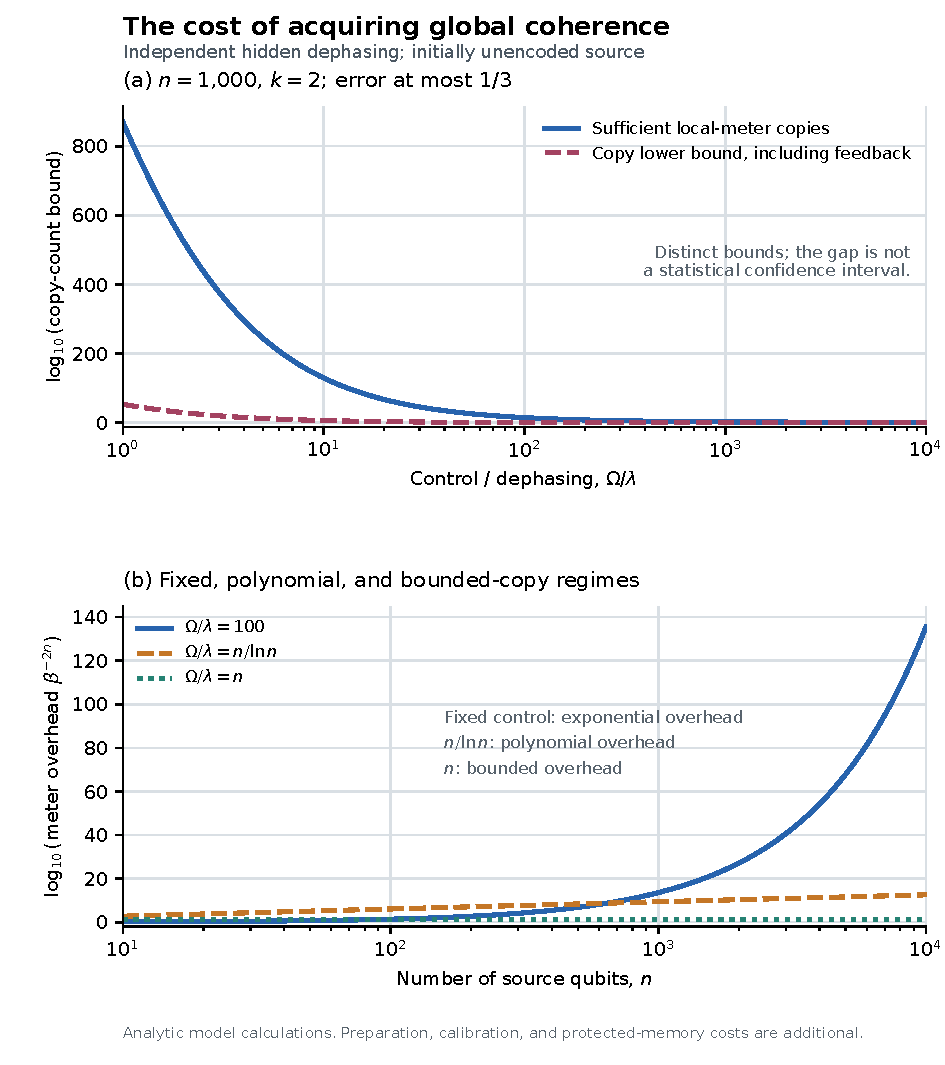
\includegraphics[width=\linewidth]{resource_law_report.pdf}
\caption{Analytic bounds and constructive costs. The lower curve covers measured feedback; the upper curve is the sufficient cost of the explicit local meter. Their gap is not a statistical confidence interval. The second panel contrasts fixed control speed with speeds proportional to $n/\ln n$ and $n$. All quantities are model calculations.}
\end{figure}

\section{What the result establishes and leaves open}

The completed statement is an all-strength acquisition limit and a matched fixed-$k$ speed/slew law for specified global-coherence promises. A larger protected processor cannot itself compensate for a fixed-speed noisy interface to those coherences.

Independent inaccessible Markov dephasing, full retained covariance of uncharged operations, and the actual summed Hamiltonian decomposition are load-bearing premises. Correlated noise, finite bath memory, available purifiers, or bath-changing controls require other analysis. An uncharged retained $X$ measurement violates the model even if its averaged source channel is covariant.

The matching reader is not a universal purity algorithm or full-state decoder. The theorem does not rule out efficient local observables, structured tasks, protected-input readout, or quantum advantages under other resources. It is not a zero-capacity theorem. The continuous-Hamiltonian pure-port recovery problem remains open here.

At growing $k$, the bound is still valid, but the fixed-$k$ matching does not extend the older weak-control conclusion for every $k=o(n)$ to all strong-control ratios. A sharp joint strong-regime law in $n,k,\Omega/\lambda$ remains open. Strict hard bandwidth and microscopic implementation are not supplied by a finite-slew control model.

This is a substantive foundational advance relative to the explicit handoff gap. A civilization-changing experimental capability has not been demonstrated. What is earned is a limitation holding at all fixed strengths, together with the resource scale at which a simple reader escapes it.

\clearpage
\appendix
\section{Sharper coefficient under a global budget}
\label{app:sharp}

With a global summed operator-norm decomposition, including coherent controllers, a sharper fixed-trajectory lemma holds:
\begin{equation}
 \boxed{\norm{\Phi_\omega(t)\Pcal_R}_\diamond
 \le A(t)^{\lceil |S|/k\rceil},\qquad0<A(t)\le1.}
 \label{eq:sharplemma}
\end{equation}
It implies the binomial certificate, for $p=1-e^{-2\lambda t}$,
\begin{align}
 \norm{\Phi(t)\Pcal_R}_\diamond
 &\le\sum_{s=0}^w\binom ws p^s(1-p)^{w-s}A(t)^{\lceil s/k\rceil}\nonumber\\
 &\le[(1-p)+pA(t)^{1/k}]^w.
\end{align}
At $A=1/2$, $t=1/(2\Omega)$, this replaces $e^{-\lambda/(k\Omega)}$ in the main coefficient by $e^{-\lambda/\Omega}$.

Introduce $x_i\in[0,1]$ for each hit site $i\in S$, and replace
\begin{equation}
 H_a(u)\longmapsto H_a(u)\prod_{\substack{i\in B_a\cap S\\u<\tau_i}}x_i.
\end{equation}
All interpolated propagators remain CPTP. If $x_i=0$, all noncommuting control on $i$ before its first dephasing is absent, so that first dephasing kills the sector.

Consider an expression consisting of physical propagator segments and exposed commutator insertions. Mark the union $C$ of their complete supports, put $U=S\setminus C$, and bound the product of insertion norms by $W$. For any unresolved $i$, the insertions commute with $\Zcal_i$ and their coefficients do not depend on $x_i$. The expression still vanishes on $x_i=0$.

Induct on $s=|U|$. With no unresolved sites the bound is $W$. Otherwise select one unresolved $i$ and integrate the derivative in $x_i$ from zero to one. Duhamel differentiation acts only on propagator segments and exposes one new term touching $i$ before $\tau_i$. Mark its entire support. The residual size $s'$ satisfies $s-k\le s'\le s-1$, so the new term is bounded by $Wh_a(u)A(t)^{\lceil s/k\rceil-1}$. The open segments partition the time interval apart from insertion instants; summing insertions costs at most $\int_0^t\sum_{a:i\in B_a}h_a(u)du\le A(t)$. This proves~\eqref{eq:sharplemma}.

This argument can expose insertions in nonchronological order. Under merely branchwise classical budgets, a later support tag must not silently choose an earlier differentiated site. A preliminary proof-tag extension did not justify that interchange. The main chronological proof was constructed to retain the full feedback scope without it. The stronger branchwise-only coefficient is not claimed.

For constant $\Omega$, the strong-control leading loss from $c=A(t)$ is $2(\lambda/\Omega)c(1-c^{1/k})$. Its optimal fixed-window choice is $c=(k/(k+1))^k$, with $c^{1/k}=k/(k+1)$. This improves constants, not the fixed-$k$ scaling conclusions.

\section{Reproducibility and governing sources}

The package contains this source/PDF, the figure program and numerical data, the separate derivation, the corrected independent proof check, the finite-trajectory program and results, a source manifest, and reproduction instructions. A separate effusion/intervention companion is preserved with its own premises and costs; the quantum theorem does not use it.

The handoff is pinned to Git revision \texttt{5cfc803599d9f95cfa0a55896fb580e77567e162}. The original P1 theorem and audit are accepted premises. The present checks concern the new theorem, not a new validation campaign for the handoff.

\begingroup
\small\setlength{\parskip}{2pt}
\begin{thebibliography}{9}
\bibitem{astra} Astra P1, \emph{A physical access theorem for quantum experiments}, supplied return, 5 November 2026. \href{https://github.com/harjassand/astra-research-knowledge/tree/5cfc803599d9f95cfa0a55896fb580e77567e162/research/returns/2026-11-05-p1-experimental-access}{Fixed governing source package}, including \texttt{package/Astra\_P1\_Quantum\_Experimental\_Access.tex} and \texttt{package/proof\_audit.txt}.
\bibitem{cotler} J. Cotler, W. Gong, and I. Kannan, \emph{Noisy quantum learning theory}, Nature Communications \textbf{17}, 6979 (2026). \href{https://doi.org/10.1038/s41467-026-73693-x}{DOI}; \href{https://arxiv.org/html/2512.10929v2}{arXiv:2512.10929v2}, Sections 2.2 and Appendix G.
\bibitem{huang} H.-Y. Huang et al., \emph{Quantum advantage in learning from experiments}, Science \textbf{376}, 1182--1186 (2022). \href{https://doi.org/10.1126/science.abn7293}{DOI}; \href{https://arxiv.org/abs/2112.00778}{arXiv:2112.00778}.
\bibitem{terhal} B. M. Terhal and G. Burkard, \emph{Fault-tolerant quantum computation for local non-Markovian noise}, Physical Review A \textbf{71}, 012336 (2005). \href{https://arxiv.org/abs/quant-ph/0402104}{arXiv:quant-ph/0402104}.
\bibitem{akp} D. Aharonov, A. Kitaev, and J. Preskill, \emph{Fault-tolerant quantum computation with long-range correlated noise}, Physical Review Letters \textbf{96}, 050504 (2006). \href{https://arxiv.org/abs/quant-ph/0510231}{arXiv:quant-ph/0510231}.
\bibitem{io} M. Christandl, O. Fawzi, and A. Goswami, \emph{Fault-tolerant quantum input/output}, \href{https://arxiv.org/abs/2408.05260v3}{arXiv:2408.05260v3} (2025 revision).
\end{thebibliography}
\endgroup
\end{document}
